\chapter{Eksperymenty numeryczne}
\label{cha:numerical_experiments}
W celu przeprowadzenia eksperymentów numerycznych zaimplementowano rozszerzony filtr Kalmana oraz filtr Kalmana Gaussa-Hermite'a. Implementację przeprowadzono w~języku Python z~wykorzystaniem otwartoźródłowej biblioteki NumPy, przeznaczonej do~szybkiego wykonywania obliczeń macierzowych. Interfejs wykonanych modułów został stworzony zgodnie z~paradygmatem programowania obiektowego. \par
\section{Systemy teoretyczne}
\label{sec:theoretical_systems}
Do~porównania działania filtrów użyto początkowo dyskretnego nieliniowego modelu systemu dynamicznego, wykorzystywanego wcześniej w~\cite{Liu} i~\cite{Germani}. Przeprowadzono 50 iteracji dla czasów 1-50 i~wykorzystano EKF oraz GHKF trzeciego stopnia do~estymacji stanu systemów.\par
Model systemu wyglądał następująco:
\begin{align}\label{eq:LiuModel1}
	&\left\{ 
	\begin{array}{l}
	x_1(t+1) = 0.8x_1(t) + x_1(t)x_2(t) + 0.1 + 0.01w_1(t) \\
	x_2(t+1) = 1.5x_2(t) - x_1(t)x_2(t) + 0.1 + 0.01w_1(t) \\
	\end{array}
	\right.\nonumber \\
	&\left\{ 
	\begin{array}{l}
	z_1(t+1) = x_1(t+1) + 0.04v_1(t+1) \\
	z_2(t+1) = x_2(t+1) + 0.04v_2(t+1)
	\end{array}
	\right.
\end{align}
gdzie szum procesu oraz szum pomiaru są nieskorelowanymi białymi szumami gaussowskimi z~następującymi rozkładami: $\boldsymbol{w}(t) \sim \mathcal{N}(\boldsymbol{0}, \boldsymbol{Q})$, $\boldsymbol{v}(t) \sim \mathcal{N}(\boldsymbol{0}, \boldsymbol{R})$, $\boldsymbol{Q}=diag(0.1, 0.2)$, $\boldsymbol{R}=diag(0.1, 0.2)$; początkowy stan systemu to: $\boldsymbol{x}(0|0) = [1,1]^T$, $\boldsymbol{P}(0|0) = \boldsymbol{I}_{2 \times 2}$.\\ 
Jako miarę skuteczności filtracji użyto pierwiastka z~błędu średniokwadratowego (ang. \textit{root-mean-square error}, RMSE), który dla $T$ estymat $\hat{x}_t$ rzeczywistych wartości $x_t$ jest definiowany następująco:
\begin{align}\label{eq:rmse}
\text{RMSE} = \sqrt{\frac{\sum_{t=1}^{T}(\hat{x}_t - x_t)^2}{T}}
\end{align}
Wykorzystanie EKF wymagało obliczenia macierzy $\boldsymbol{G}$ i $\boldsymbol{H}$:
\begin{align}\label{eq:LiuModel1GH}
\boldsymbol{G}&=
\begin{bmatrix}
x_2 + 0.8 & x_1 \\
-x_2 & 1.5 - x_1
\end{bmatrix} \nonumber \\
\boldsymbol{H}&=\boldsymbol{I}_{2 \times 2}
\end{align}
Dla EKF wartość RMSE wyniosła, odpowiednio dla $x_1$ i~$x_2$, 0.01244 i~0.01042, natomiast dla GHKF 0.01246 oraz 0.00961. Rysunek \ref{fig:Liu1_errors} przedstawia wykresy różnic pomiędzy wartością estymowaną, a~rzeczywistą dla zmiennych stanu badanego systemu. Oba algorytmy dobrze poradziły sobie z~postawionym problemem, wartości błędów były bardzo niewielkie, a~różnice między wartościami wyjściowymi algorytmów minimalne.   
\begin{figure}
	\centering
	\begin{subfigure}[b]{0.4\linewidth}
		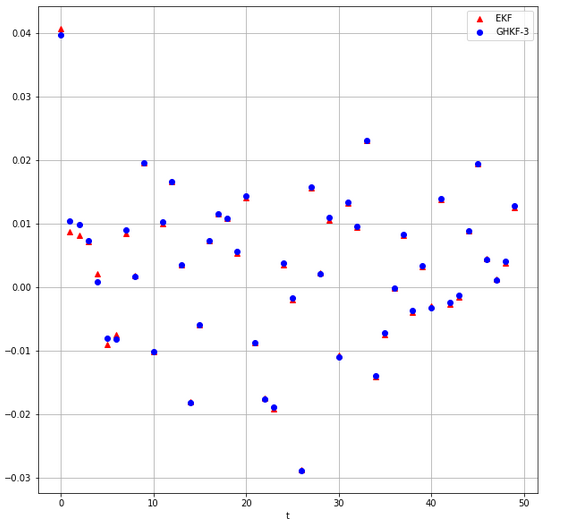
\includegraphics[width=\linewidth]{Liu1_x1_error.png}
		\caption{}
		\label{fig:Liu1_errors_a}
	\end{subfigure}
	\begin{subfigure}[b]{0.4\linewidth}
		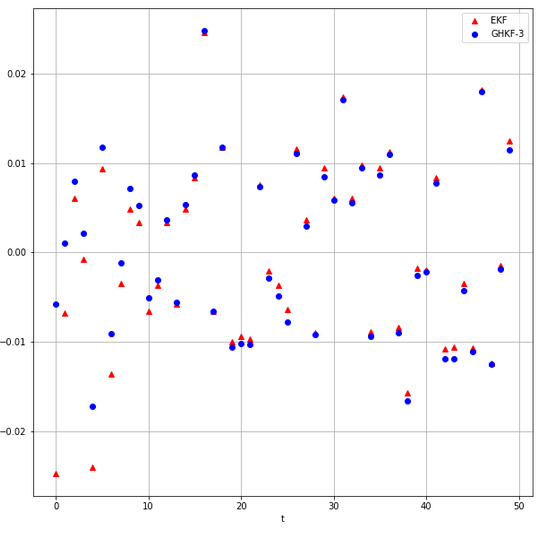
\includegraphics[width=\linewidth]{Liu1_x2_error.png}
		\caption{}
		\label{fig:Liu1_errors_b}
	\end{subfigure}
	\caption{Różnice między wartością estymowaną, a rzeczywistą dla $x_1$(\ref{fig:Liu1_errors_a}) oraz $x_2$ (\ref{fig:Liu1_errors_b}).}
	\label{fig:Liu1_errors}
\end{figure}


\par


W~celu dokładniejszego zbadania, jak nieliniowość funkcji wpływa na~działanie obu rodzajów filtrów, przeprowadzono testy dla następującej rodziny systemów:
\begin{align}\label{eq:rmseTestModel}
x(t+1) &= x(t) + a\sin(2x(t)) + w(t) \nonumber \\
z(t+1) &= x(t+1) + v(t+1)
\end{align}
$a\in{0..20}$, $w(t) \sim \mathcal{N}(0, Q)$, $v(t) \sim \mathcal{N}(0, R)$. Model procesu staje się bardziej nieliniowy dla większych wartości parametru $a$ (Rysunek \ref{fig:rmse_test_functions}). \par
Dla każdej wartości parametru $a$ wykonano 100 iteracji algorytmów rozszerzonego filtru Kalmana oraz filtru Kalmana Gaussa-Hermite'a stopnia 2, 3 i 5. Każda iteracja zakładała wykonanie 100 kroków predykcji-korekcji przy zastosowaniu danego algorytmu, którego działanie było oceniane za~pomocą wartości wskaźnika RMSE. Zbadano również średni czas potrzebny na~wykonanie zadania dla poszczególnych filtrów. W~celu uzyskania takich samych wartości z~generatora liczb losowych dla każdego filtra, przed uruchomieniem symulacji generator był inicjowany tym samym zarodkiem. Przyjęto następujące wartości parametrów symulacji i~filtracji: $Q=10$, $R=10$, $x(0|0)=1$, $P(0|0)=1$. \par
\begin{figure}[h!]
	\centering
	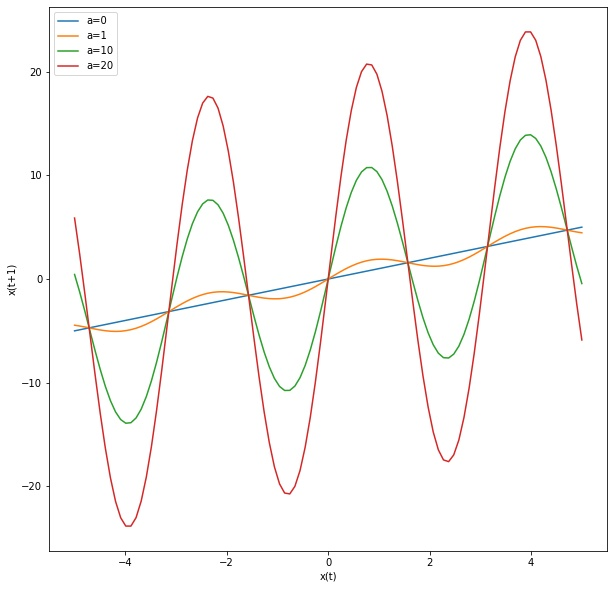
\includegraphics[width=0.5\linewidth]{rmse_test_functions.jpg}
	\caption{Funkcje w modelu procesu użyte do przetestowania działania filtrów dla kilku wartości parametru $a$}
	\label{fig:rmse_test_functions}
\end{figure}
Na~rysunku \ref{fig:rmse_test_results} pokazano średnie wartości RMSE dla różnych rodzajów filtrów. Dla parametru $a=0$ modele procesu oraz pomiarów są modelami liniowymi i~rezultaty filtracji były takie same. Dla innych wartości $a$ w~działaniu filtrów można zaobserwować różnice. Z~postawionym zadaniem najlepiej poradził sobie filtr Kalmana Gaussa-Hermite'a stopnia 3, uzyskując najniższe średnie wartości RMSE dla każdego $a$. Rozszerzony filtr Kalmana uzyskiwał RMSE gorsze o około 0.45 dla bardziej nieliniowych modeli. Dwupunktowa aproksymacja wykorzystywana przez GHKF-2 okazała się mało dokładna i~dla $a>10$ uzyskane wyniki są zdecydowanie najsłabsze. Zwiększenie liczby węzłów do~5 również nie przyniosło poprawy wyników - rezultaty uzyskane przez GHKF-5 są zbliżone do~GHKF-3 dla $a>12$, natomiast dla mniejszych $a$ są nawet gorsze. \par
Średni czas na~wykonanie postawionego zadania nieco różnił się dla poszczególnych filtrów (Tabela \ref{tab:rmse_times}). Najszybszy był rozszerzony filtr Kalmana, natomiast w~przypadku filtru Kalmana Gaussa-Hermite'a im więcej węzłów było wykorzystywanych, tym średni czas był większy.
\begin{figure}[h!]
	\centering
	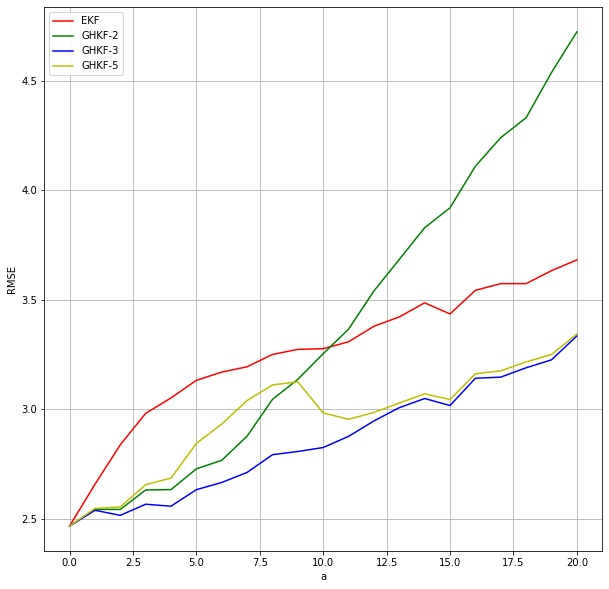
\includegraphics[width=0.8\linewidth]{rmse_test_results.jpg}
	\caption{Średnie wartości RMSE dla testowanych filtrów dla różnych wartości parametru $a$}
	\label{fig:rmse_test_results}
\end{figure}
\begin{table}[]
	\caption{Względne średnie czasy działania algorytmów}
	\label{tab:rmse_times}
	\begin{center}
		\begin{tabular}{|l|l|l|l|}
			\hline
			\textbf{EKF} & \textbf{GHKF-2} & \textbf{GHKF-3} & \textbf{GHKF-5} \\ 
			\hline
			1 & 1.037 & 1.05 & 1.08 \\
			\hline
		\end{tabular}
	\end{center}
\end{table}

\section{Problemy praktyczne}
\label{sec:practical_problems}

\subsection{Śledzenie pocisku balistycznego}
\label{subsec:ballistic_target_tracking}
Problem śledzenia pocisku balistycznego jest kluczowy dla skutecznego przechwycania pocisku, co ma duże znaczenie dla kwestii bezpieczeństwa i~obronności. Rozważany jest scenariusz, kiedy pocisk balistyczny ponownie wchodzi w~atmosferę Ziemi po~przemierzeniu dużego dystansu, jego prędkość jest bardzo duża, a~czas do uderzenia w ziemię stosunkowo niewielki. Problem ten jest uznawany za trudny ze względu na: szum pomiaru, nieliniowości w~modelu procesu lub pomiaru oraz brak informacji o~kształcie i~wielkości pocisku. \cite{MisslieTracking1}\cite{MissileTracking2}.
\begin{figure}[h!]
	\centering
	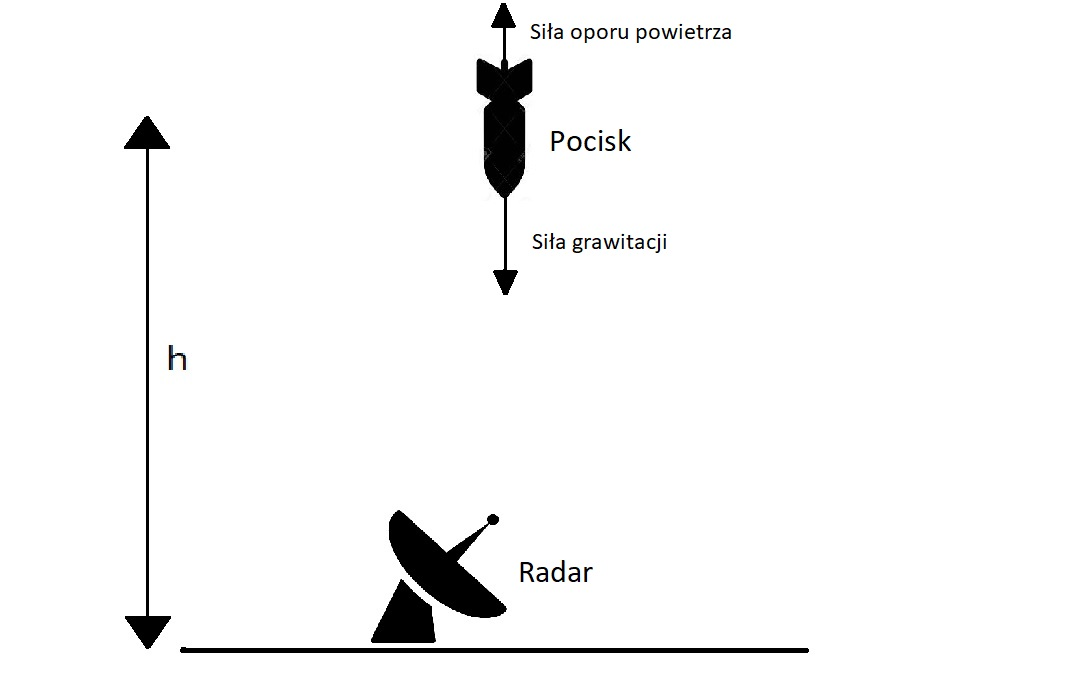
\includegraphics[width=0.8\linewidth]{missile_tracking_illustration.jpg}
	\caption{Scenariusz śledzenia pocisku balistycznego przez radar umieszczony na ziemi}
	\label{fig:missile_tracking_illustration}
\end{figure}
\par
Założono, że pocisk spada pionowo na~ziemię, tak jak pokazano na rysunku \ref{fig:missile_tracking_illustration}, opór powietrza i~grawitacja działają w~linii prostej, siła nośna działająca na~pocisk jest pomijalnie mała, ziemia jest płaska i~stacjonarna, a~grawitacja nie zależy od wysokości. Bazując na~powyższych założeniach, ruch obiektu można opisać następującymi równaniami \cite{MissileTrackingEquations}:
\begin{align}\label{eq:missile_tracking_model}
\dot{h} &= -v \nonumber \\
\dot{v} &= - \frac{\rho(h)gv^2}{2\beta} + g \nonumber \\
\dot{\beta} &= 0
\end{align}
gdzie $g$ to przyspieszenie ziemskie ($9.81\,m/s^2$), $h$ to wysokość, na~jakiej znajduje się pocisk (w $m$), $v$ to prędkość pocisku ($m/s$), natomiast jako $\beta$ oznaczony jest współczynnik balistyczny. Gęstość powietrza $\rho(h)=a_1e^{-a_2h}$ jest wykładniczą funkcją wysokości, gdzie $a_1=1.754$ i~$a_2=1.49\cdot10^{-4}$.
Po~dyskretyzacji i~po uwzględnionieniu szumu model procesu dla wektora zmiennych stanu $\boldsymbol{x}=\begin{bmatrix}
h & v & \beta
\end{bmatrix}^T$ wygląda następująco:
\begin{align}\label{eq:missile_tracking_discretized_model}
	h(t+1) &= h(t) - v(t)T + w_1(t) \nonumber \\
	v(t+1) &= v(t)-\frac{\rho(h(t))gv(t)^2}{2\beta(t)}T + gT + w_2(t) \nonumber \\
	\beta(t+1) &= \beta(t) + w_3(t)
\end{align}
Ze~względu na~siłę oporu powietrza, dynamika obiektu jest silnie nieliniowa. Szum procesu $\boldsymbol{w}(t)$ jest szumem gaussowskim o~średniej $\boldsymbol{0}$ i~macierzy kowariancji $\boldsymbol{Q}$,
\begin{equation}
\boldsymbol{Q} = 
	\begin{bmatrix}
	q_3T^3/3 & q_3T^2/2 & 0 \\
	q_3T^2/2 & q_3T & 0 \\
	0 & 0 & q_4T
	\end{bmatrix}
\end{equation}
gdzie parametry $q_3$ (w~$m^2/s^3$) oraz $q_4$ (w~$kg^2m^{-2}s^{-5}$) należy dostroić dla konkretnego systemu. \par
Na rysunku \ref{fig:ballistic_typical_trajectories} przedstawiono typowe przebiegi wysokości oraz prędkości pocisku niezakłócone szumem procesu ($q_3=q_4=0$). Przez kilka początkowych sekund prędkość nie zmienia się znacząco. Potem jednak gęstość powietrza zwiększa się i~siła oporu spowalnia spadający obiekt. W~końcu pocisk uzyskuje stałą prędkość, kiedy siła grawitacji i~opór powietrza równoważą się. Początkowe wartości wysokości, prędkości i~współczynnika balistycznego ustawiono odpowiednio na~$60960\,m$, $3048\,m/s$ i~$19161\,kg/ms^2$. Czas próbkowania $T$ wynosił $0.1\,s$.\par
\begin{figure}
	\centering
	\begin{subfigure}[b]{0.4\linewidth}
		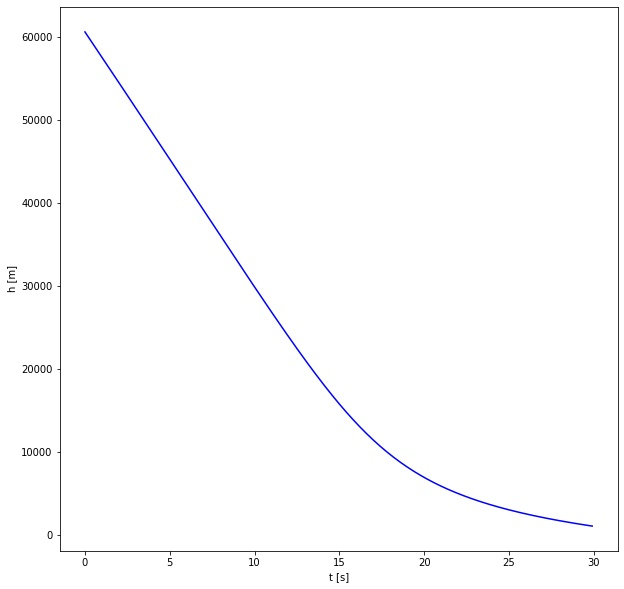
\includegraphics[width=\linewidth]{ballistic_tracking_typical_h.jpg}
		\caption{}
		\label{fig:ballistic_typical_trajectories_h}
	\end{subfigure}
	\begin{subfigure}[b]{0.4\linewidth}
		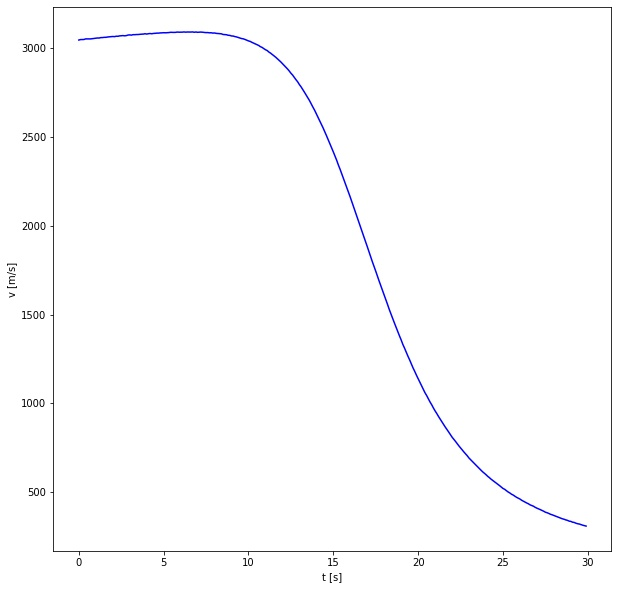
\includegraphics[width=\linewidth]{ballistic_tracking_typical_v.jpg}
		\caption{}
		\label{fig:ballistic_typical_trajectories_v}
	\end{subfigure}
	\caption{Typowe przebiegi wysokości (\ref{fig:ballistic_typical_trajectories_h}) oraz prędkości (\ref{fig:ballistic_typical_trajectories_v}) pocisku}
	\label{fig:ballistic_typical_trajectories}
\end{figure}
Pozycja pocisku jest mierzona przy użyciu radaru umieszczonego na~ziemi. Model pomiaru jest modelem liniowym, zakłócanym przez szum gaussowski o średniej $0$ i wariancji $R$.
\begin{equation}
z(t+1) = \boldsymbol{H}\boldsymbol{x}(t+1) + \nu(t+1)
\end{equation}
gdzie $\boldsymbol{H} = \begin{bmatrix}
1 & 0 & 0
\end{bmatrix}$ \par
Powyższy problem został rozwiązany przy użyciu rozszerzonego filtru Kalmana oraz filtru Kalmana Gaussa-Hermite'a. Parametry szumu procesu dla filtrów oraz symulacji ustalono podobnie jak w~\cite{MisslieTracking1} na $q_3=q_4=5$. Wartość wariancji szumu pomiarowego przyjęto jako $R=200^2$. Na~rysunku \ref{fig:ballistic_errors} przedstawiono różnice pomiędzy prawdziwymi wartościami wysokości pocisku, prędkości oraz współczynnika balistycznego, a~estymatami wyznaczonymi przez filtry. Oba filtry dobrze poradziły sobie z~postawionym problemem. Błędy w~oszacowaniu wysokości pocisku wynosiły kilkadziesiąt metrów przez większą część trwania symulacji, równocześnie nie przekraczając $200\,m$. Po~początkowej rozbieżności w~estymacie prędkości sięgającej $180\, m/s$, błąd w~oszacowaniu zmalał i~do~końca symulacji utrzymywał się na niskim poziomie. Estymowane wartości współczynnika balistycznego również były zbliżone do~prawdziwych. Wyniki otrzymywane przy użyciu obu filtrów są niemal identyczne. Dla opisanego problemu śledzenia pocisku balistycznego, linearyzacja funkcji występującej w~modelu procesu, wykorzystywana przez rozszerzony filtr Kalmana, jest dokładna.
\begin{figure}
	\centering
	\begin{subfigure}[b]{0.4\linewidth}
		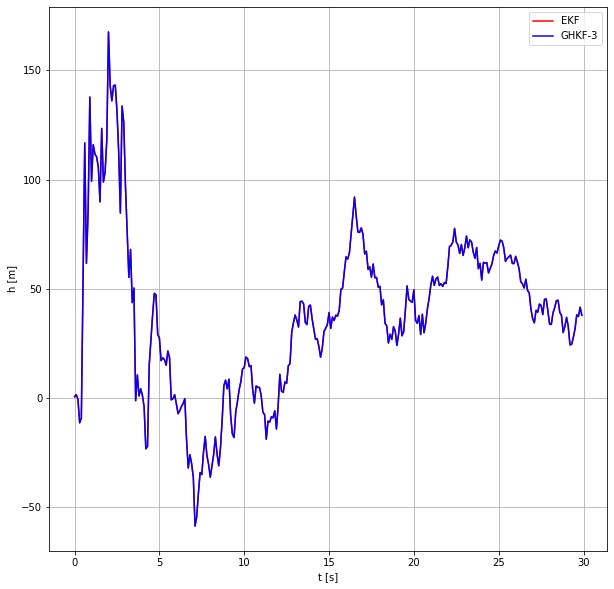
\includegraphics[width=\linewidth]{ballistic_tracking_h_errors.jpg}
		\caption{}
		\label{fig:ballistic_errors_h}
	\end{subfigure}
	\begin{subfigure}[b]{0.4\linewidth}
		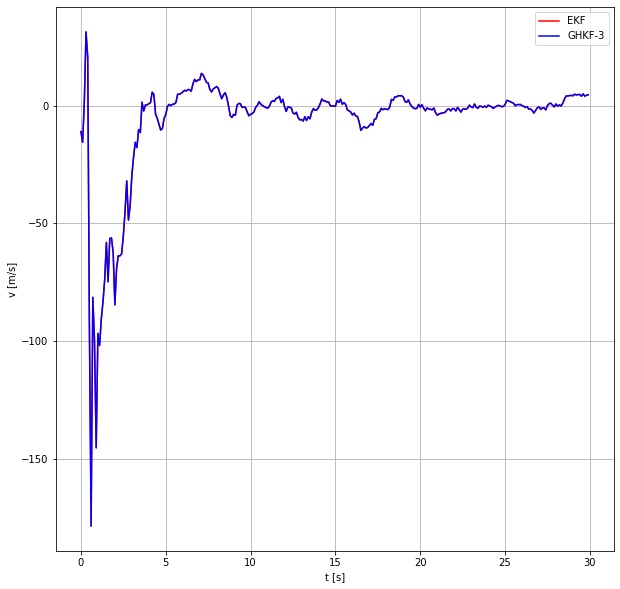
\includegraphics[width=\linewidth]{ballistic_tracking_v_errors.jpg}
		\caption{}
		\label{fig:ballistic_errors_v}
	\end{subfigure}
	\begin{subfigure}[b]{0.4\linewidth}
	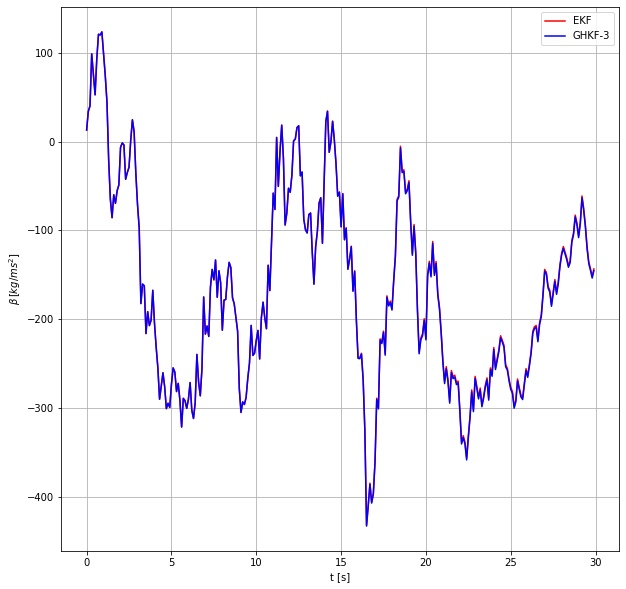
\includegraphics[width=\linewidth]{ballistic_tracking_b_errors.jpg}
	\caption{}
	\label{fig:ballistic_errors_b}
	\end{subfigure}
	\caption{Różnice pomiędzy wartością prawdziwą, a~estymowaną przez filtry dla wysokości (\ref{fig:ballistic_errors_h}), prędkości (\ref{fig:ballistic_typical_trajectories_v}) oraz współczynnika balistycznego (\ref{fig:ballistic_errors_b})}
	\label{fig:ballistic_errors}
\end{figure}
\subsection{Dwuwymiarowe śledzenie ruchu obiektu}
\label{subsec:2D_target_tracking}
W~przypadku problemu dwuwymiarowego śledzenia ruchu obiektu pozycja celu jest opisywana przy użyciu kartezjańskiego układu współrzędnych, natomiast pomiary są uzyskiwane w~układzie współrzędnych biegunowych. Przyjmując wektor stanu $\boldsymbol{x}=\begin{bmatrix}
x & v_x & a_x & y & v_y & a_y
\end{bmatrix}^T$ model procesu wygląda następująco \cite{Konatowski_2D_Tracking}:
\begin{align}\label{eq:2D_tracking_process_model}
x(t+1) &= x(t)+Tv_x(t)+0.5T^2a_x(t)+w_1(t) \nonumber \\
v_x(t+1) &= v_x(t)+Ta_x(t)+w_2(t) \nonumber \\
a_x(t+1) &= a_x(t)+w_3(t) \nonumber \\
y(t+1) &= y(t)+Tv_y(t)+0.5T^2a_y(t)+w_4(t) \nonumber \\
v_y(t+1) &= v_y(t)+Ta_y(t)+w_5(t) \nonumber \\
a_y(t+1) &= a_y(t)+w_6(t)
\end{align}
gdzie $\boldsymbol{w}_t\sim\mathcal{N}(\boldsymbol{0}, \boldsymbol{Q})$, $T$ - okres próbkowania.\par
Model pomiarowy przyjmuje ogólną postać
\begin{equation}
\boldsymbol{z}(t+1) = \boldsymbol{h}(\boldsymbol{x}(t+1)) + \boldsymbol{v}(t+1)
\end{equation}
gdzie $\boldsymbol{v} \sim \mathcal{N}(\boldsymbol{0}, \boldsymbol{R})$, natomiast nieliniowa funkcja $\boldsymbol{h}(\boldsymbol{x}(t))$ wygląda następująco:
\begin{equation} 
\boldsymbol{h}(\boldsymbol{x}(t))=\begin{bmatrix}
\rho(t) & \theta(t)
\end{bmatrix}^T = \begin{bmatrix}
\sqrt{x(t)^2 + y(t)^2} & \arctan(\frac{x(t)}{y(t)})
\end{bmatrix}^T
\end{equation}
dla mierzonych wartości dystansu $\rho(t)$ oraz azymutu $\theta(t)$. \par
Podczas testów symulacyjnych wykonanych dla $100\,s$ przyjęto następujące wartości parametrów: $\boldsymbol{P}(0|0) = \boldsymbol{I}_{6 \times 6}$, $\boldsymbol{x}(0|0)=\begin{bmatrix}
200\,m & 50\,\frac{m}{s} & 15\,\frac{m}{s^2} & 100\,m & 80\,\frac{m}{s} & 20\,\frac{m}{s^2}
\end{bmatrix}^T$, $\boldsymbol{R}=diag(10, 0.03)$, $T=1\,s$. Macierz kowariancji szumu procesu $\boldsymbol{Q}=diag(0,0,1000,0,0,1000)$ wykorzystywana przez filtry została podana w~formie uproszczonej \cite[247]{labbe2014}. Podobnie jak w~\cite{Konatowski_2D_Tracking} w~symulacji ruchu obiektu przyjęto, że śledzony cel wykonuje skręt w~lewo, odejmując w~każdym kroku od~składowej $x$ przyspieszenia $5\,\frac{m}{s^2}$ dla $t<50\,s$. \par
Na rysunku \ref{fig:2D_tracking_positions} przedstawiono położenie śledzonego obiektu oraz wyniki estymacji położenia wykonane przez rozszerzony filtr Kalmana oraz filtr Kalmana Gaussa-Hermite'a stopnia 2 i~3. Rysunek \ref{fig:2D_tracking_errors} przedstawia z~kolei różnice pomiędzy rzeczywistymi wartościami zmiennych stanu, a estymatami wyznaczonymi przez filtry. Najlepiej z~postawionym zadaniem poradził sobie filtr Kalmana Gaussa-Hermite'a stopnia trzeciego, estymując wszystkie zmienne stanu z~niewielkim błędem przez cały czas trwania symulacji. Rozszerzony filtr Kalmana słabo poradził sobie z~estymacją położenia podczas zmiany przyspieszenia, która nie była uwzględniona w~modelu procesu. Estymowane wartości składowych $x$ prędkości i~przyspieszenia na~koniec symulacji mocno odbiegały od~wartości rzeczywistych. Dwupunktowa aproksymacja rozkładów używana przez GHKF-2 również okazała się mało dokładna i,~podobnie jak w~przypadku EKF, różnice pomiędzy wartościami rzeczywistymi, a~estymowanymi są znaczące. Dla postawionego problemu badano również filtr Kalmana Gaussa-Hermite'a stopnia 5, jednak uzyskiwane wyniki były niemal identyczne jak w~przypadku GHKF-3. \par
Czasy potrzebne do~estymacji stanu przy użyciu róznych filtrów przedstawiono w tabeli \ref{tab:2D_tracking_times}. Pomiędzy algorytmami występowały znaczące różnice wynikające z~dużej liczby zmiennych stanu w~badanym problemie. Najkrótszy czas wystąpił dla rozszerzonego filtru Kalmana, natomiast dla algorytmów Gaussa-Hermite'a wzrastał bardzo szybko wraz ze~wzrostem stopnia algorytmu i~ostatecznie GHKF-5 okazał się ponad 300 razy wolniejszy od~EKF. 
\begin{table}[]
	\caption{Względne czasy działania algorytmów dla problemu dwuwymiarowego śledzenia obiektu}
	\label{tab:2D_tracking_times}
	\begin{center}
		\begin{tabular}{|l|l|l|l|}
			\hline
			\textbf{EKF} & \textbf{GHKF-2} & \textbf{GHKF-3} & \textbf{GHKF-5} \\ 
			\hline
			1 & 2.36 & 14.82 & 330 \\
			\hline
		\end{tabular}
	\end{center}
\end{table}
\begin{figure}
	\centering
	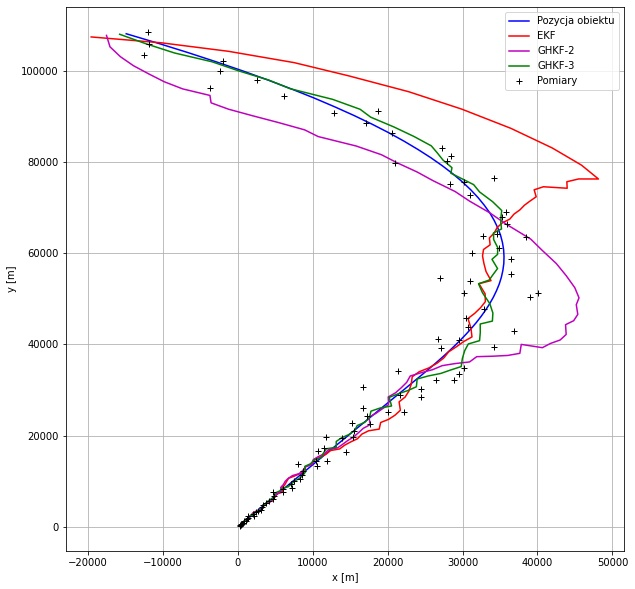
\includegraphics[width=\linewidth]{2D_tracking_positions.jpg}
	\caption{Położenie obiektu estymowane przez filtry}
	\label{fig:2D_tracking_positions}
\end{figure}
\begin{figure}
	\centering
	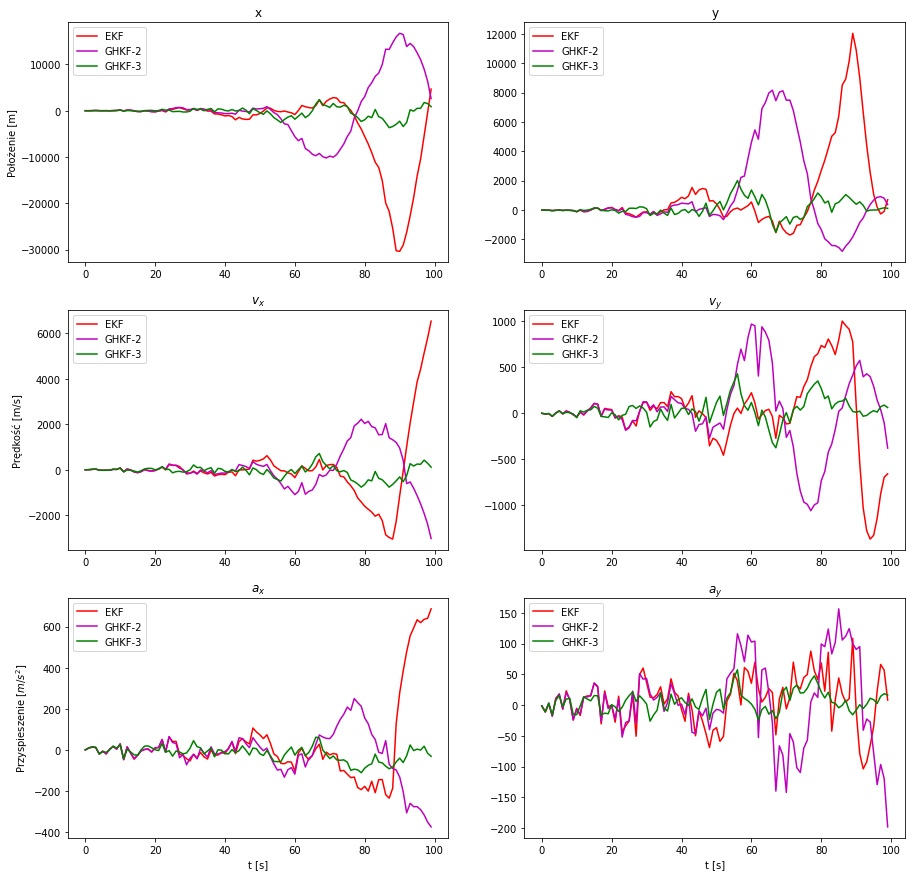
\includegraphics[width=\linewidth]{2D_tracking_errors.jpg}
	\caption{Różnice pomiędzy rzeczywistymi wartościami zmiennych stanu, a estymowanymi przez filtry}
	\label{fig:2D_tracking_errors}
\end{figure}
\subsection{Śledzenie wyłącznie z wykorzystaniem namiaru}
\label{subsec:bot}
Śledzenie wyłącznie z~wykorzystaniem namiaru (ang. \textit{Bearing only tracking}, BOT) to problem ważny w~wielu praktycznych zastosowaniach, zarówno wojskowych, jak i~cywilnych, np. w~systemach broni podwodnej, nawigacji robotów przy użyciu sonaru, nadzorze nad ruchem lotniczym z~wykorzystaniem radaru pasywnego, czy śledzeniu ruchu ludzi przy użyciu sygnału z~kamery lub mikrofonu. Celem BOT jest śledzenie kinematyki poruszającego się obiektu przy użyciu pomiaru kąta pomiędzy kierunkiem odniesienia, a~kierunkiem, w~którym obserwowany jest obiekt namierzany. Nieliniowość występująca w~systemie oraz problem z~obserwowalnością czynią śledzenie wyłącznie z~wykorzystaniem namiaru problemem trudnym i~często pojawiającym się w~badaniach \cite{BOT_Chalasani}\cite{BOT_Arulampalam}. \par
Problem BOT wymaga kilku stacji śledzących ze~znanymi współrzędnymi lub poruszającej się platformy, której prędkość jest znana i~na~której znajduje się urządzenie śledzące. Podobnie jak w~\cite{BOT_Chalasani}, w~pracy wykorzystano system drugiego typu. Założono, że cel porusza się w~linii prostej w~osi X w~płaszczyźnie poziomej ze~stałą prędkością obarczoną szumem. W~celu śledzenia obiektu, ponad celem w~tej samej płaszczyźnie pionowej porusza się platforma, której prędkość również jest stała i~zaszumiona (rysunek \ref{fig:BOT_illustration}). 
\begin{figure}
	\centering
	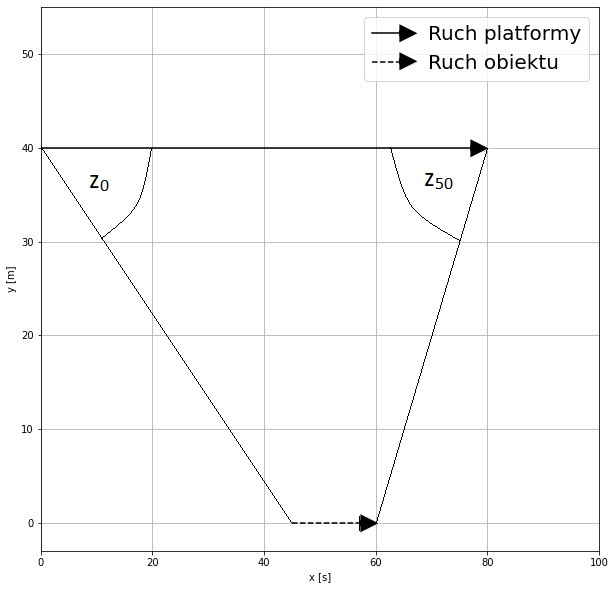
\includegraphics[width=0.7\linewidth]{BOT_illustration.jpg}
	\caption{Ilustracja badanego problemu śledzenia z~wykorzystaniem namiaru}
	\label{fig:BOT_illustration}
\end{figure}
Model procesu badanego problemu jest modelem liniowym:
\begin{align}\label{eq:BOT_process_model}
x_1(t+1) &= x_1(t) + Tx_2(t) + w_1(t) \nonumber \\
x_2(t+1) &= x_2(t) + w_2(t)
\end{align}
gdzie $x_1$ to położenie obiektu, $x_2$ - prędkość obiektu, $T=0.01\,s$ - okres próbkowania, $\boldsymbol{w} \sim \mathcal{N}(\boldsymbol{0}, \boldsymbol{Q})$, $\boldsymbol{Q}=diag(0.1, 0.1)$ \par
Ruch platformy śledzącej może być opisany za~pomocą następujących dyskretnych równań:
\begin{align}\label{eq:BOT_platform_equations}
x_p(t) &= \bar{x}_p(t) + \Delta x_p(t) \nonumber \\
y_p(t) &= \bar{y}_p + \Delta y_p(t)
\end{align}
gdzie $\bar{x}_p(t)$ i~$\bar{y}_p(t)$ są średnimi współrzędnymi pozycji platformy, a~$\Delta x_p(t)$ i~$\Delta y_p(t)$ są wzajemnie niezależnymi szumami gaussowskimi z~zerową średnią i~wariancjami odpowiednio $r_x=1\,m^2$ i~$r_y=1\,m^2$. Średnie współrzędne platformy to $\bar{x}_p(t)=160tT$ i~$\bar{y}_p(t)=40$. \par
Model pomiarowy zakłada pomiar jedynie namiaru do~obiektu:
\begin{align}\label{eq:BOT_measurement_model}
z(t) &= \arctan \frac{y_p(t)}{x_1(t) - x_p(t)} + v_s(t)
\end{align}
$v_s(t)$ to gaussowski szum pomiarowy o~zerowej średniej i~wariancji $r_s$, przy założeniu jego niezależności od~zakłóceń ruchu platformy oraz okresu próbkowania. \par
Losowy komponent ruchu platformy wpływa na~dodatkowy nieaddytywny szum pomiarowy obecny w~równaniu \ref{eq:BOT_measurement_model}. Powyższy efekt może być przybliżony szumem addytywnym poprzez przedstawienie nieliniowej funkcji modelu pomiarowego jako: 
\begin{align}\label{eq:BOT_measurement_model_approximation}
z(t) &\approx \arctan \frac{\bar{y}_p(t)}{x_1(t) - \bar{x}_p(t)} + v(t) 
\end{align}
gdzie $v(t)$ jest odpowiadającym szumem addytywnym z~wariancją $R(t)$:
\begin{equation}
\label{eq:BOT_R_matrix}
R(t) = \frac{\bar{y}_p(t)^2 r_x + (x_1(t) - \bar{x}_p(t))^2 r_y}{((x_1(t) - \bar{x}_p)^2 + \bar{y}_p^2)^2} + r_s
\end{equation} 
Przedstawiony system jest bardzo podobny do~systemu badanego w~\cite{BOT_Chalasani}. Największą różnicą jest taki dobór parametrów, by w~pewnej chwili platforma śledząca znalazła się nad śledzonym obiektem. 
\par
Opisany problem został rozwiązany przy użyciu algorytmów rozszerzonego filtru Kalmana oraz filtru Kalmana Gaussa-Hermite'a dla 50 kroków predykcji-korekcji. Jako wartości początkowe przyjęto $\boldsymbol{x}(0|0)=\begin{bmatrix}
45 & 30
\end{bmatrix}^T$, $\boldsymbol{P}(0|0) = \boldsymbol{I}_{2 \times 2}$. Na rysunku \ref{fig:BOT_results_1} przedstawiono wyniki filtracji dla wariancji szumu pomiarowego $r_s = (0.105\,rad)^2$. W~początkowej fazie symulacji zarówno rozszerzony filtr Kalmana, jak i~filtr Kalmana Gaussa-Hermite'a stopnia trzeciego dobrze radziły sobie z~estymacją pozycji obiektu. W~dalszej fazie wyniki uzyskiwane za~pomocą EKF stają się mocno niedokładne. Niedokładność ma związek z~punktową linearyzacją funkcji wykorzystywaną przez EKF. Na~rysunku \ref{fig:BOT_h_function} przedstawiono wykres funkcji występującej w~modelu pomiarowym systemu. Aproksymacja funkcji staje się trudna dla położenia obiektu $x$ zbliżonego do~położenia platformy $\bar{x}_p$ i~rozszerzony filtr Kalmana błędnie oszacowuje wynikowy rozkład. Oszacowanie EKF staje się poprawne przy zwiększeniu przekazywanej do~filtra wariancji szumu pomiarowego (rysunek \ref{fig:BOT_results_2}). W~przypadku zmniejszenia wariancji szumu, oba filtry dają błędne wyniki, tak jak przedstawiono na~rysunku \ref{fig:BOT_results_3}. W~tej sytuacji brak rozbieżności filtru można uzyskać stosując dokładniejszą aproksymację rozkładu za~pomocą algorytmu Kalmana Gaussa-Hermite'a stopnia piątego.
\begin{figure}
	\centering
	\begin{subfigure}[b]{0.4\linewidth}
		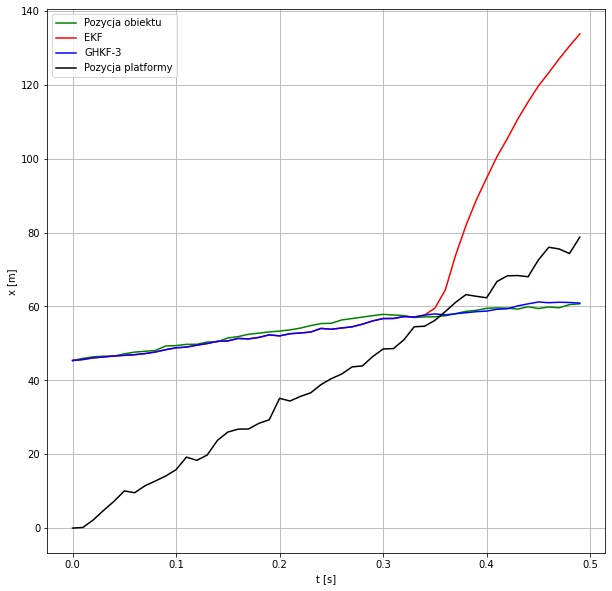
\includegraphics[width=\linewidth]{BOT_results_1.jpg}
		\caption{}
		\label{fig:BOT_results_1}
	\end{subfigure}
	\begin{subfigure}[b]{0.4\linewidth}
		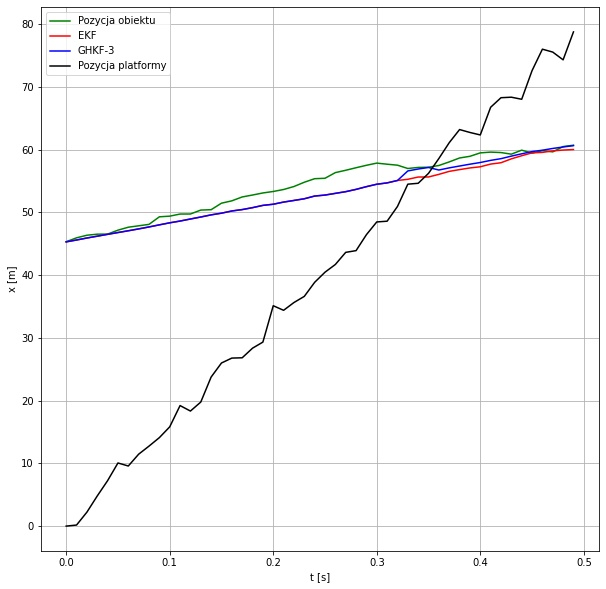
\includegraphics[width=\linewidth]{BOT_results_2.jpg}
		\caption{}
		\label{fig:BOT_results_2}
	\end{subfigure}
	\begin{subfigure}[b]{0.4\linewidth}
		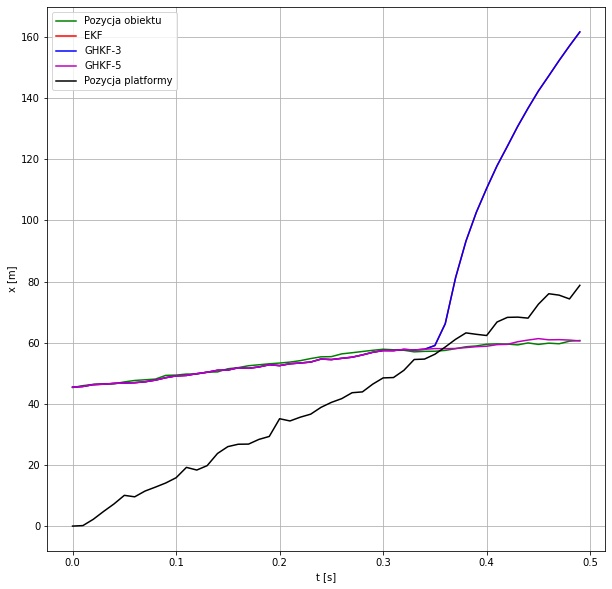
\includegraphics[width=\linewidth]{BOT_results_3.jpg}
		\caption{}
		\label{fig:BOT_results_3}
	\end{subfigure}
	\caption{Wyniki estymacji położenia dla $r_s = (0.105\,rad)^2$ (\ref{fig:BOT_results_1}), $r_s = (1\,rad)^2$ (\ref{fig:BOT_results_2}), $r_s = (0.052\,rad)^2$ (\ref{fig:BOT_results_3})}
	\label{fig:BOT_results}
\end{figure}
\begin{figure}
	\centering
	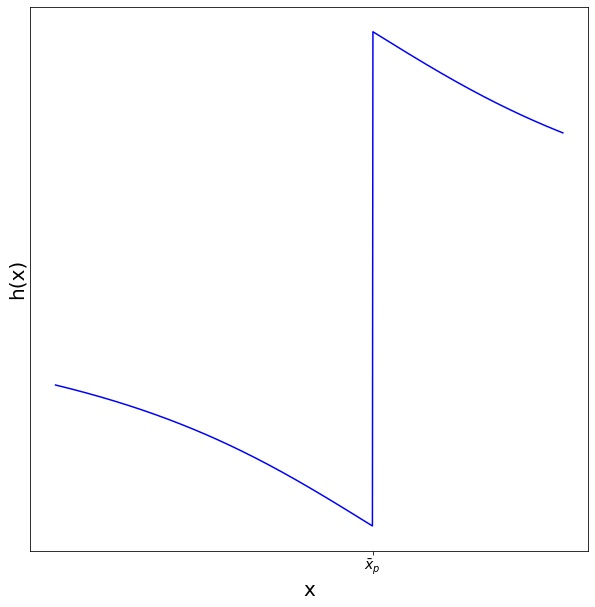
\includegraphics[width=0.4\linewidth]{BOT_h_function.jpg}
	\caption{Wykres funkcji $h(x) = \arctan \frac{\bar{y}_p}{x - \bar{x}_p}$ używanej w~modelu pomiarowym systemu} 
	\label{fig:BOT_h_function}
\end{figure}

